\chapter{Introducció}

L'objectiu principal d'aquest informe és l'estudi de l'aerodinàmica d'un planejador i l'efecte que té sobre ella l'efecte terra. Per tal de poder resoldre el problema plantejat, s'utilitza el mètode numèric de Vortex lattice.

Es comença analitzant l'aerodinàmica de l'ala aïllada per poder estudiar com es troba influenciada pels paràmetres geomètrics, i, un cop determinada la geometria final de l'ala, es procedeix a analitzar l'efecte sòl.

A continuació, s'afegeixen els estabilitzadors vertical i horitzontal i, de nou, se n'estudia els coeficients aerodinàmics. També s'afegeix l'anàlisi de moments. Finalment, es realitza l'anàlisi del planejador complet amb efecte terra.

\begin{figure}[h]
	\centering
	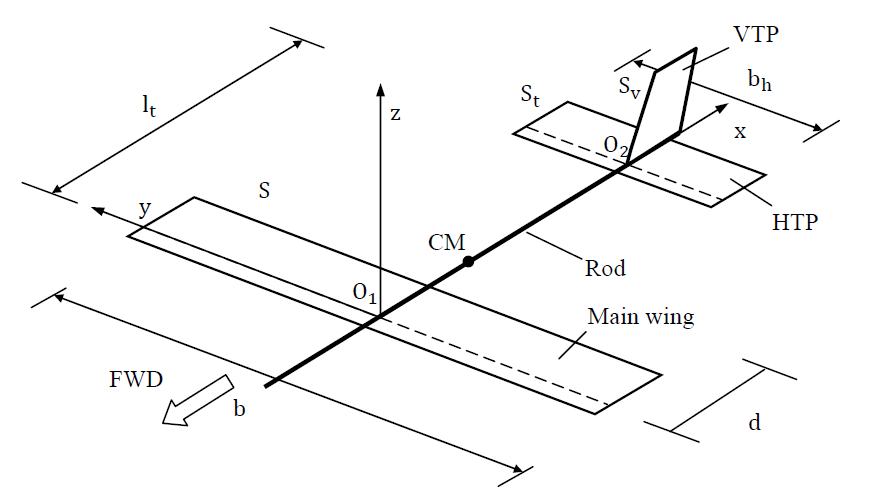
\includegraphics[scale=0.5]{plots/enunciat.png}
	\caption{Esquema del planejador}
	\label{enunciat}
\end{figure}

L'esquema del planejador, així com els paràmetres geomètrics i els eixos de referència utilitzats, es troben definits en la figura \ref{enunciat}. Les relacions entre alguns d'aquests paràmetres estan fixats per les següents expressions:
\begin{itemize}
	\item $\frac{S_{t}}{S}=\frac{1}{8}$
	\item $\frac{S_{v}}{S}=\frac{2}{3}$
	\item $\frac{l_{t}}{\bar{c}}=4$
\end{itemize}

Per tal de definir els paràmetres bàsics de la geometria de l'ala del planejador, s'ha agafat com a referència l'avió SZD-56 Diana 2 de Diana Sailplanes \cite{Kubrynski2006}. Els valors determinats són:
\begin{itemize}
	\item $\lambda=0.3$
	\item $A=26$
	\item $\Lambda=0$
	\item $\Gamma=0$
\end{itemize}

% Falta posar coses de geometria dels estabilitzadors crec, però aquests valors no sé quins són :s

En quant als perfils utilitzats, en l'ala s'assumeix un perfil NACA 2412 i en els estabilitzadors vertical i horitzontal, NACA 0009.